
\begin{figure}[H]
    \centering
    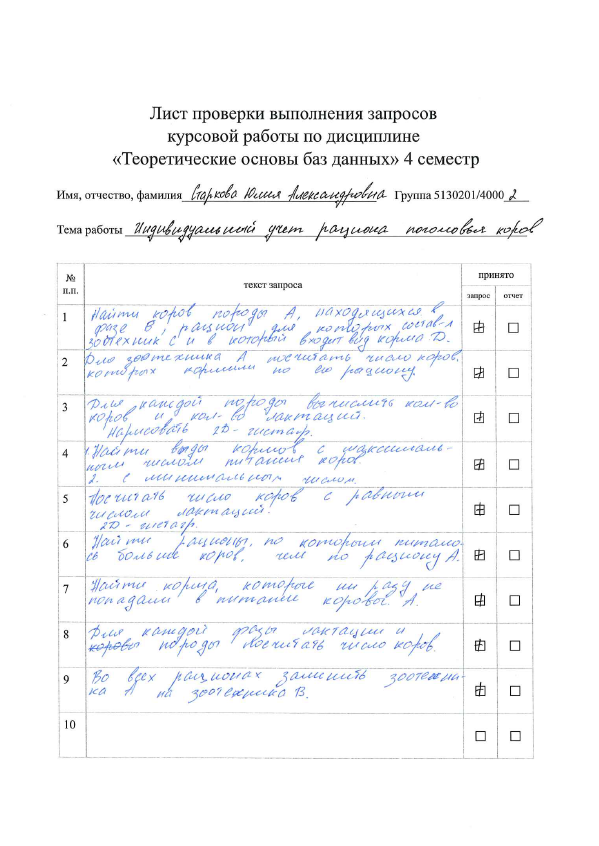
\includegraphics[width=1\linewidth]{Программирование/запросы_скан2.png}
\end{figure}
\subsection{Запрос 1}
\textbf{Формулировка запроса на русском языке.}
Найти коров породы A, находящихся в фазе лактации B, рацион для которых составлял зоотехник C и в который входит вид корма D.

Текст запроса на SQL приведен в листинге \ref{lst:1}.
\listingcaption{Текст запроса 1 на SQL}\label{lst:1}
\begin{Verbatim}[numbers=left, frame=single, breaklines=true, breakanywhere=true]
SELECT DISTINCT Cow.id_Cow, Breed.Name AS Breed_Name, Lactation_Phase.Name AS Lactation_Phase_Name, 
Livestock_specialist.First_name, 
Livestock_specialist.Surname, Feed_type.Name AS Feed_type_Name
FROM Cow
JOIN Breed ON Cow.id_Breed = Breed.id_Breed
JOIN Lactation ON Cow.id_Cow = Lactation.id_Cow
JOIN Lactation_Phase ON Lactation.id_Lactation_Phase = Lactation_Phase.id_Lactation_Phase
JOIN Diet ON Lactation_Phase.id_Lactation_Phase = Diet.id_Lactation_Phase
JOIN Livestock_specialist ON Diet.id_Livestock_specialist = Livestock_specialist.id_Livestock_specialist
JOIN Feeding_plan ON Diet.id_Diet = Feeding_plan.id_Diet
JOIN Feeds ON Feeding_plan.id_Feeds = Feeds.id_Feeds
JOIN Feed_type ON Feeds.id_Feed_type = Feed_type.id_Feed_type
WHERE Breed.Name = 'Рязанская'
  AND Lactation_Phase.Name = 'Середина лактации'
  AND Livestock_specialist.First_name = 'Артем' 
  AND Livestock_specialist.Surname = 'Новиков'
  AND Feed_type.Name = 'Солома';
\end{Verbatim}
На рисунке \ref{fig:1} представлен результат выполнения запроса 1 (часть таблицы).
\begin{figure}[H]
    \centering
    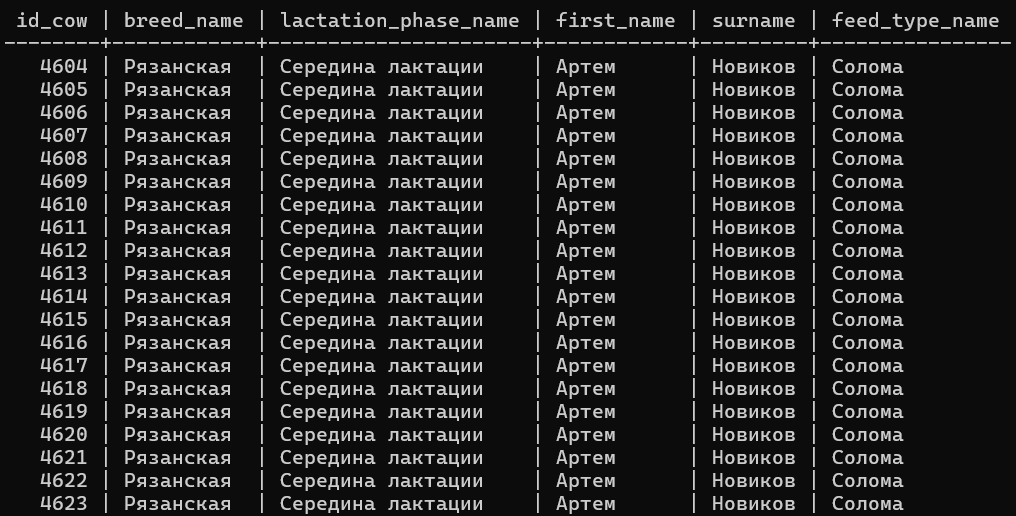
\includegraphics[width=0.9\linewidth]{результаты запросов/1(b).png}
    \caption{Результат выполнения запроса 1}
    \label{fig:1}
\end{figure}
Количество записей после выполнения запроса составило 657.
\textbf{Время выполнения запроса: }957.662 ms.

На картинке \ref{fig:дер1} представлено графическое представление последовательности выполнения запроса 1.
\clearpage
\newgeometry{margin=1cm}
\begin{landscape}
    \begin{figure}[p]
        \centering
        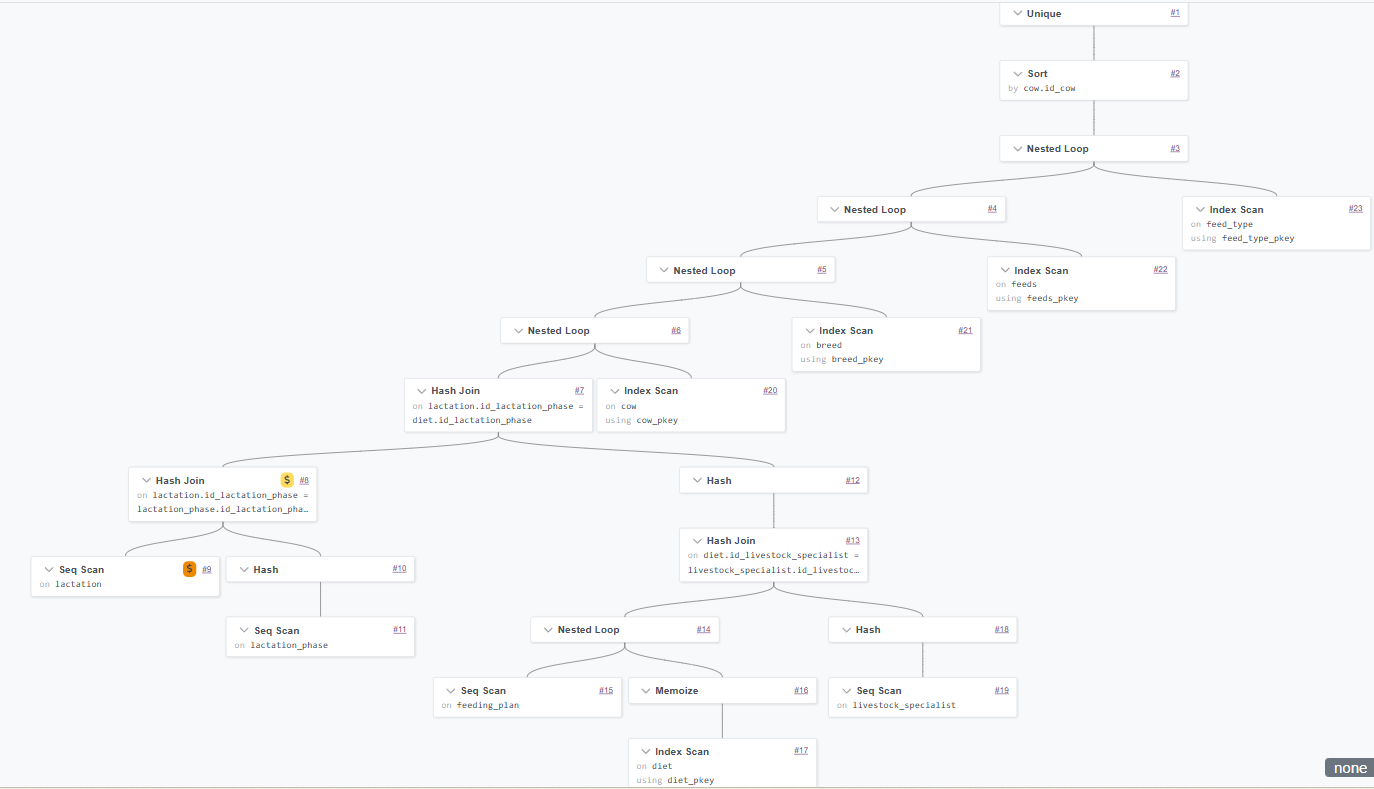
\includegraphics[width=\linewidth, height=\textheight, keepaspectratio]{деревья/дерево1.png}
        \caption{Графическое представление последовательности выполнения запроса 1}
        \label{fig:дер1}
    \end{figure}
\end{landscape}
\restoregeometry
\clearpage

\textbf{Текстовое объяснение последовательности выполнения запроса 1.}\\
В запросе последовательно соединяются таблицы \texttt{Cow, Breed, Lactation, Lactation\_Phase, Diet, Livestock\_specialist, Feeding\_plan, Feeds и Feed\_type} с помощью оператора \texttt{JOIN}. Затем с помощью \texttt{WHERE} выбираются строки, значения которых совпадают с указанными в запросе: порода коровы --- <<Рязанская>>, фаза лактации --- <<Середина лактации>>, имя и фамилия зоотехника --- <<Артем Новиков>>, вид корма --- <<Солома>>. После фильтрации с помощью ключевого слова \texttt{DISTINCT} удаляются дублирующиеся строки.

\textbf{Реляционная формула запроса.}
\[
\pi_{\text{cow.id\_Cow},\, \text{breed.Name},\, \text{lp.Name},\, \text{ls.First\_name},\, \text{ls.Surname},\, \text{ft.Name}} (
\]

\[
\sigma_{\substack{
\text{breed.Name}{=}\text{`Рязанская'} \wedge\, \text{lp.Name}{=}\text{`Середина лактации'} \wedge \\
\text{ls.First\_name}{=}\text{`Артем'} \wedge\, \text{ls.Surname}{=}\text{`Новиков'} \wedge\, \text{ft.Name}{=}\text{`Солома'}
}}
(
\]

\[
\text{Cow} \bowtie_{\text{cow.id\_Breed}=\text{breed.id\_Breed}} \text{Breed}
\]
\[
\bowtie_{\text{cow.id\_Cow}=\text{lact.id\_Cow}} \text{Lactation}
\]
\[
\bowtie_{\text{lact.id\_Lactation\_phase}=\text{lp.id\_Lactation\_phase}} \text{Lactation\_Phase}
\]
\[
\bowtie_{\text{lp.id\_Lactation\_phase}=\text{diet.id\_Lactation\_phase}} \text{Diet}
\]
\[
\bowtie_{\text{diet.id\_Livestock\_specialist}=\text{ls.id\_Livestock\_specialist}} \text{Livestock\_specialist}
\]
\[
\bowtie_{\text{diet.id\_Diet}=\text{fp.id\_Diet}} \text{Feeding\_plan}
\]
\[
\bowtie_{\text{fp.id\_Feeds}=\text{feeds.id\_Feeds}} \text{Feeds}
\]
\[
\bowtie_{\text{feeds.id\_Feed\_type}=\text{ft.id\_Feed\_type}} \text{Feed\_type}))
\]


\subsection{Запрос 2}
\textbf{Формулировка запроса на русском языке.}
Для зоотехника A посчитать число коров, которых кормили по его рациону.

Текст запроса на SQL приведен в листинге \ref{lst:2}.
\listingcaption{Текст запроса 2 на SQL}\label{lst:2}
\begin{Verbatim}[numbers=left, frame=single, breaklines=true, breakanywhere=true]
SELECT COUNT(DISTINCT Nutrition.id_Cow) 
FROM Livestock_specialist 
JOIN Diet ON Livestock_specialist.id_Livestock_specialist = Diet.id_Livestock_specialist
JOIN Feeding_plan ON Diet.id_Diet = Feeding_plan.id_Diet
JOIN Nutrition ON Feeding_plan.id_Feeding_plan = Nutrition.id_Feeding_plan
WHERE Livestock_specialist.Surname = 'Смирнова' 
  AND Livestock_specialist.First_name = 'Екатерина';
\end{Verbatim}
На рисунке \ref{fig:2} представлен результат выполнения запроса 2.
\begin{figure}[H]
    \centering
    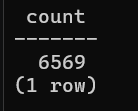
\includegraphics[width=0.25\linewidth]{результаты запросов/2.png}
    \caption{Результат работы запроса 2}
    \label{fig:2}
\end{figure}
\textbf{Время выполнения запроса: }35.705 ms.

На картинке \ref{fig:дерево2} представлено графическое представление последовательности выполнения запроса 2.
\begin{figure}[H]
    \centering
    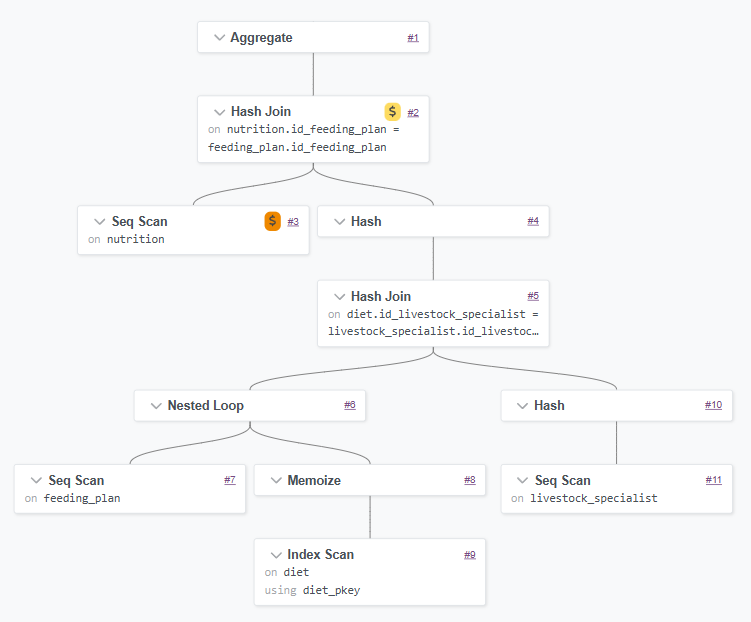
\includegraphics[width=1\linewidth]{деревья/дерево2.png}
    \caption{Графическое представление последовательности выполнения запроса 2}
    \label{fig:дерево2}
\end{figure}

\textbf{Текстовое объяснение последовательности выполнения запроса 2.}\\
В запросе последовательно соединяются таблицы \texttt{Livestock\_specialist, Diet, Feeding\_plan} и \texttt{Nutrition} с помощью оператора \texttt{JOIN}. Затем с помощью \texttt{WHERE} выбираются строки, значения которых совпадают с указанными в запросе: имя и фамилия зоотехника --- <<Екатерина Смирнова>>. После фильтрации с помощью агрегатной функции \texttt{COUNT} и ключевого слова \texttt{DISTINCT} вычисляется количество уникальных идентификаторов коров, которые питались по планам кормления, составленным данным зоотехником.

\textbf{Реляционная формула запроса.}
\[
\mathcal{G}_{\text{COUNT(DISTINCT n.id\_Cow)} \rightarrow \text{cow\_count}} (
\]

\[
\sigma_{\substack{
\text{ls.Surname}{=}\text{`Смирнова'} \wedge\, \text{ls.First\_name}{=}\text{`Екатерина'}
}} (
\]

\[
\text{Livestock\_specialist} \bowtie_{\text{ls.id\_Livestock\_specialist}=\text{diet.id\_Livestock\_specialist}} \text{Diet}
\]
\[
\bowtie_{\text{diet.id\_Diet}=\text{fp.id\_Diet}} \text{Feeding\_plan}
\]
\[
\bowtie_{\text{fp.id\_Feeding\_plan}=\text{n.id\_Feeding\_plan}} \text{Nutrition}))
\]

\newpage
\subsection{Запрос 3}
\textbf{Формулировка запроса на русском языке.}
Для каждой породы вычислить количество коров и количество количество лактаций.

Текст запроса приведен в листинге \ref{lst:3}.
\listingcaption{Текст запроса 3 на SQL}\label{lst:3}
\begin{Verbatim}[numbers=left, frame=single, breaklines=true, breakanywhere=true]
SELECT 
    Breed.Name AS Breed_name, 
    COUNT(DISTINCT Cow.id_Cow) AS Cow_count,  
    COUNT(Lactation.id_Lactation) AS Lactation_count 
FROM Breed 
LEFT JOIN Cow ON Breed.id_Breed = Cow.id_Breed
LEFT JOIN Lactation ON Cow.id_Cow = Lactation.id_Cow
GROUP BY Breed.id_Breed, Breed.Name;
\end{Verbatim}
На рисунке \ref{fig:3} представлен результат выполнения запроса 3.
\begin{figure}[H]
    \centering
    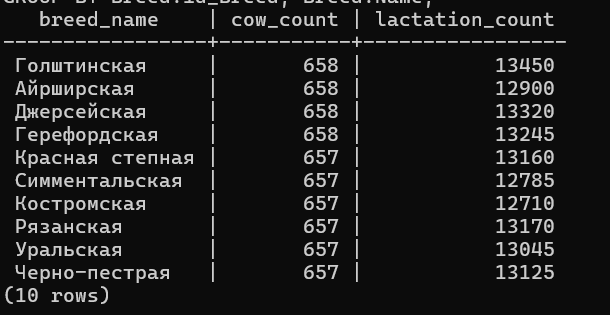
\includegraphics[width=1\linewidth]{результаты запросов/3.png}
    \caption{Результат работы запроса 3}
    \label{fig:3}
\end{figure}

\textbf{Время выполнения запроса: }128.959 ms.

На картинке \ref{fig:дер3} представлено графическое представление последовательности выполнения запроса 3.
\begin{figure}[H]
    \centering
    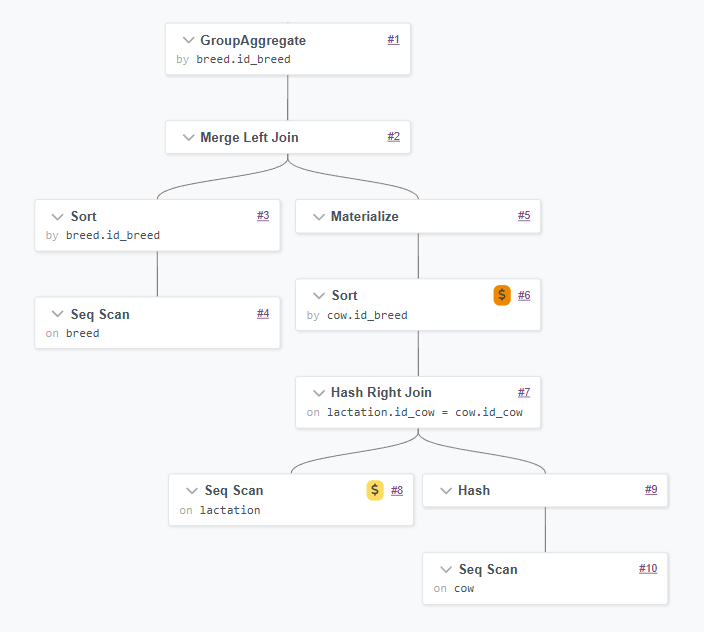
\includegraphics[width=0.75\linewidth]{деревья/дерево3.png}
    \caption{Графическое представление последовательности выполнения запроса 3}
    \label{fig:дер3}
\end{figure}

\textbf{Текстовое объяснение последовательности выполнения запроса 3.}\\
В запросе к таблице \texttt{Breed} последовательно присоединяются таблицы \texttt{Cow} и \texttt{Lactation} с помощью оператора внешнего левого соединения \texttt{LEFT JOIN}, что позволяет сохранить в выборке породы, для которых в базе данных пока нет записей о коровах. Затем строки группируются по идентификатору и названию породы с помощью \texttt{GROUP BY}. После группировки с помощью агрегатной функции \texttt{COUNT} и ключевого слова \texttt{DISTINCT} вычисляется количество уникальных коров для каждой породы, а с помощью функции \texttt{COUNT} --- общее количество зарегистрированных лактаций.

На рисунке \ref{fig:гист3} представлена 2d-гистограмма результатов запроса 3.
\begin{figure}[H]
    \centering
    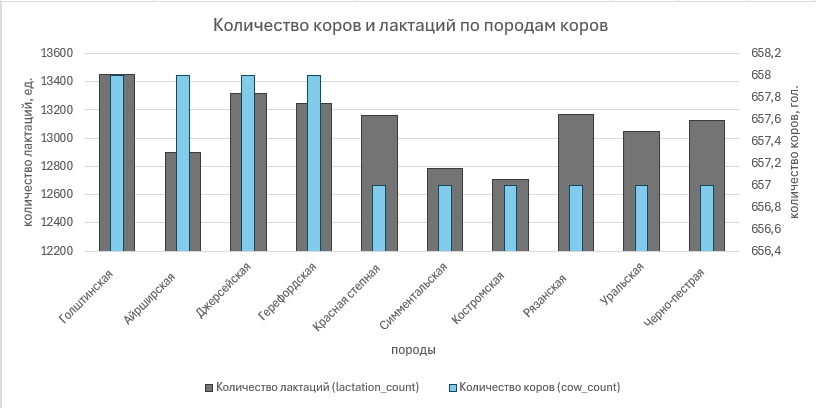
\includegraphics[width=0.75\linewidth]{гистаграммы/гистагр3.png}
    \caption{Распределение количества коров и лактаций для каждой породы}
    \label{fig:гист3}
\end{figure}

\textbf{Реляционная формула запроса.}
\[
\mathcal{G}_{\substack{
\text{breed.id\_Breed},\, \text{breed.Name}, \\
\text{COUNT(DISTINCT cow.id\_Cow)}{\rightarrow}\text{cow\_count}, \\
\text{COUNT(lact.id\_Lactation)}{\rightarrow}\text{lactation\_count}
}}
\left( \text{Breed} \underset{\text{breed.id\_Breed}=\text{cow.id\_Breed}}{\overset{\text{LEFT}}{\bowtie}} \text{Cow} \underset{\text{cow.id\_Cow}=\text{lact.id\_Cow}}{\overset{\text{LEFT}}{\bowtie}} \text{Lactation} \right)
\]

\subsection{Запрос 4}
\textbf{Запрос 4.1}

\textbf{Формулировка запроса на русском языке.}
Найти виды кормов с максимальным числом питания коров.

\listingcaption{Текст запроса 4.1 на SQL}\label{lst:4.1}
\begin{Verbatim}[numbers=left, frame=single, breaklines=true, breakanywhere=true]
SELECT Feed_type.Name AS Feed_type_Name, COUNT(DISTINCT Nutrition.id_Cow) AS Cow_count
FROM Feed_type
JOIN Feeds ON Feed_type.id_Feed_type = Feeds.id_Feed_type
JOIN Feeding_plan ON Feeds.id_Feeds = Feeding_plan.id_Feeds
JOIN Nutrition ON Feeding_plan.id_Feeding_plan = Nutrition.id_Feeding_plan
GROUP BY Feed_type.id_Feed_type, Feed_type.Name
HAVING COUNT(DISTINCT Nutrition.id_Cow) = (
    SELECT MAX(cow_count) FROM (
        SELECT COUNT(DISTINCT Nutrition.id_Cow) AS cow_count
        FROM Feed_type
        JOIN Feeds ON Feed_type.id_Feed_type = Feeds.id_Feed_type
        JOIN Feeding_plan ON Feeds.id_Feeds = Feeding_plan.id_Feeds
        JOIN Nutrition ON Feeding_plan.id_Feeding_plan = Nutrition.id_Feeding_plan
        GROUP BY Feed_type.id_Feed_type
    ) AS counts
);
\end{Verbatim}
На рисунке \ref{fig:4.1} представлен результат выполнения запроса 4.1.
\begin{figure}[H]
    \centering
    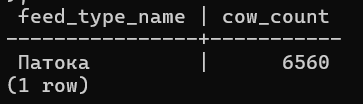
\includegraphics[width=0.5\linewidth]{результаты запросов/4.1.png}
    \caption{Результат работы запроса 4.1}
    \label{fig:4.1}
\end{figure}

\textbf{Время выполнения запроса: }450.523 ms.

На картинке \ref{fig:дер4.1} представлено графическое представление последовательности выполнения запроса 4.1.
\clearpage
\newgeometry{margin=1cm}
\begin{landscape}
    \begin{figure}[p]
        \centering
        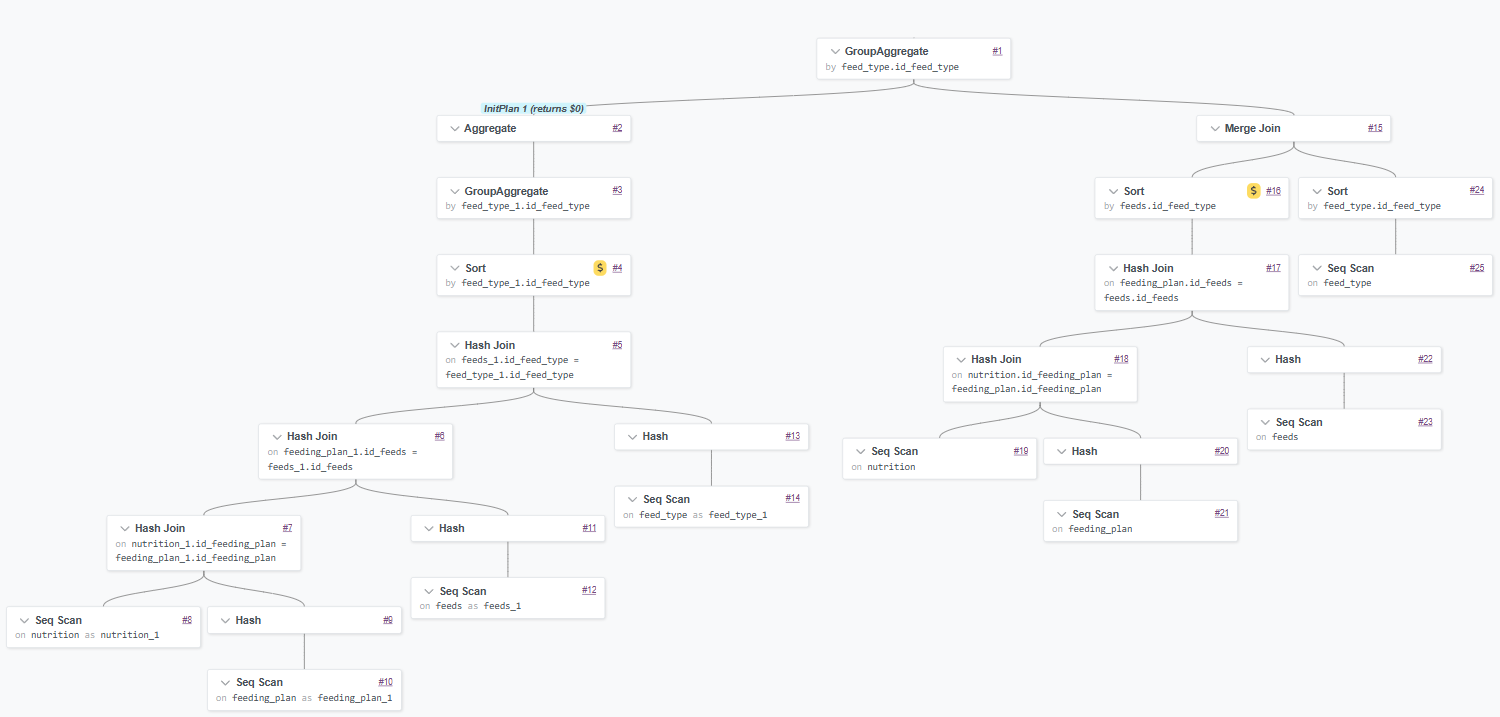
\includegraphics[width=\linewidth, height=\textheight, keepaspectratio]{деревья/дерево4.1.png}
        \caption{Графическое представление последовательности выполнения запроса 4.1}
        \label{fig:дер4.1}
    \end{figure}
\end{landscape}
\restoregeometry
\clearpage

\textbf{Текстовое объяснение последовательности выполнения запроса 4.1.}\\
В запросе последовательно соединяются таблицы \texttt{Feed\_type, Feeds, Feeding\_plan} и \texttt{Nutrition} с помощью оператора \texttt{JOIN}. Затем строки группируются по идентификатору и названию типа корма, а с помощью функций \texttt{COUNT}, \texttt{GROUP BY} и ключевого слова \texttt{DISTINCT} вычисляется количество уникальных коров, которые питались каждым типом корма. С помощью условия \texttt{HAVING} полученное количество коров сравнивается с результатом подзапроса, который находит максимальное значение (\texttt{MAX}) количества коров среди всех типов кормов. В результате выводятся только те виды кормов, которые имеют максимальное число уникальных коров в питании.

\textbf{Реляционная формула запроса.}
\[
\sigma_{\text{cow\_count} = \text{MAX(cow\_count)}} (
\]
\[
\mathcal{G}_{\substack{
\text{ft.id\_Feed\_type},\, \text{ft.Name}, \\
\text{COUNT(DISTINCT n.id\_Cow)}{\rightarrow}\text{cow\_count}
}} (
\]
\[
\text{Feed\_type} \bowtie_{\text{ft.id\_Feed\_type}=\text{f.id\_Feed\_type}} \text{Feeds}
\]
\[
\bowtie_{\text{f.id\_Feeds}=\text{fp.id\_Feeds}} \text{Feeding\_plan}
\]
\[
\bowtie_{\text{fp.id\_Feeding\_plan}=\text{n.id\_Feeding\_plan}} \text{Nutrition}))
\]

\textbf{Запрос 4.2}

\textbf{Формулировка запроса на русском языке.}
Найти виды кормов с минимальным числом питания коров.

\listingcaption{Текст запроса 4.2 на SQL}\label{lst:4.2}
\begin{Verbatim}[numbers=left, frame=single, breaklines=true, breakanywhere=true]
SELECT Feed_type.Name AS Feed_type_Name, COUNT(DISTINCT Nutrition.id_Cow) AS cow_count
FROM Feed_type
JOIN Feeds ON Feed_type.id_Feed_type = Feeds.id_Feed_type
JOIN Feeding_plan ON Feeds.id_Feeds = Feeding_plan.id_Feeds
JOIN Nutrition ON Feeding_plan.id_Feeding_plan = Nutrition.id_Feeding_plan
GROUP BY Feed_type.id_Feed_type, Feed_type.Name
HAVING COUNT(DISTINCT Nutrition.id_Cow) = (
    SELECT MIN(cow_count)
    FROM (
        SELECT COUNT(DISTINCT Nutrition.id_Cow) AS cow_count
        FROM Feed_type
        JOIN Feeds ON Feed_type.id_Feed_type = Feeds.id_Feed_type
        JOIN Feeding_plan ON Feeds.id_Feeds = Feeding_plan.id_Feeds
        JOIN Nutrition ON Feeding_plan.id_Feeding_plan = Nutrition.id_Feeding_plan
        GROUP BY Feed_type.id_Feed_type
    ) AS counts
);
\end{Verbatim}
На рисунке \ref{fig:4.2} представлен результат выполнения запроса 4.2.
\begin{figure}[H]
    \centering
    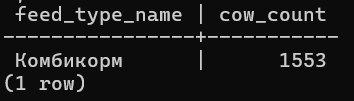
\includegraphics[width=0.5\linewidth]{результаты запросов/4.2.png}
    \caption{Результат работы запроса 4.2}
    \label{fig:4.2}
\end{figure}
\textbf{Время выполнения запроса: }443.040 ms.

На картинке \ref{fig:дер4.2} представлено графическое представление последовательности выполнения запроса 4.2.
\clearpage
\newgeometry{margin=1cm}
\begin{landscape}
    \begin{figure}[p]
        \centering
        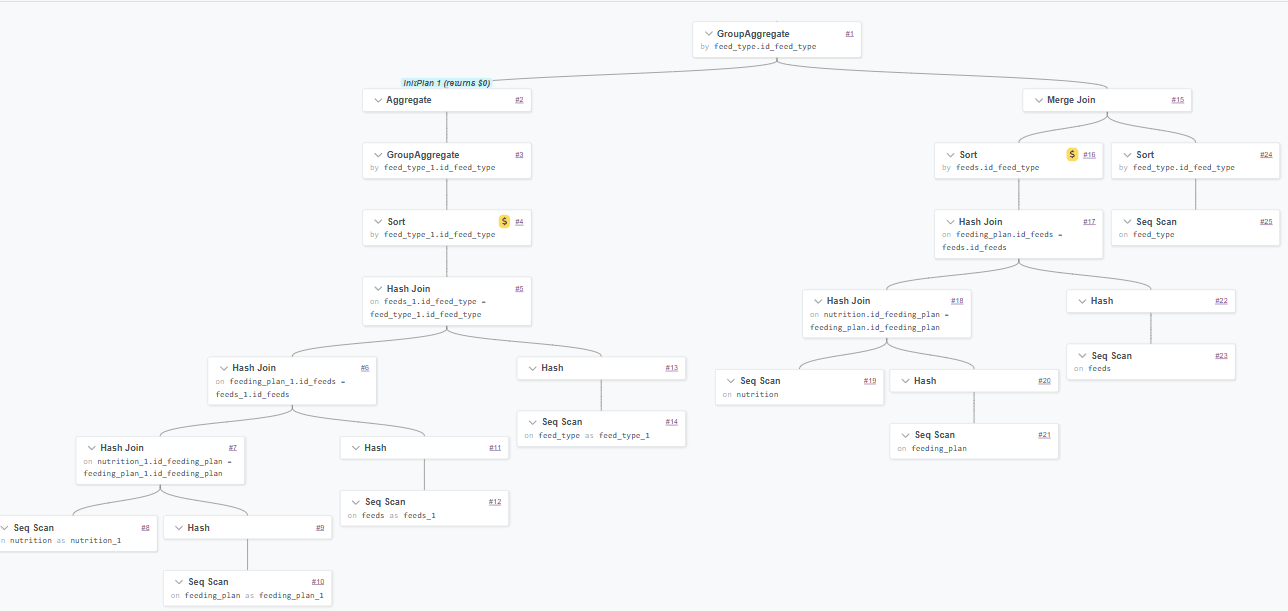
\includegraphics[width=\linewidth, height=\textheight, keepaspectratio]{деревья/дерево4.2.png}
        \caption{Графическое представление последовательности выполнения запроса 4.2}
        \label{fig:дер4.2}
    \end{figure}
\end{landscape}
\restoregeometry
\clearpage

\textbf{Текстовое объяснение последовательности выполнения запроса 4.2.}\\
В запросе последовательно соединяются таблицы \texttt{Feed\_type, Feeds, Feeding\_plan} и \texttt{Nutrition} с помощью оператора \texttt{JOIN}. Затем строки группируются по идентификатору и названию типа корма, а с помощью функций \texttt{COUNT}, \texttt{GROUP BY} и ключевого слова \texttt{DISTINCT} вычисляется количество уникальных коров, которые питались каждым типом корма. С помощью условия \texttt{HAVING} полученное количество коров сравнивается с результатом подзапроса, который находит максимальное значение (\texttt{MIN}) количества коров среди всех типов кормов. В результате выводятся только те виды кормов, которые имеют максимальное число уникальных коров в питании.

\textbf{Реляционная формула запроса.}
\[
\sigma_{\text{cow\_count} = \text{MIN(cow\_count)}} (
\]
\[
\mathcal{G}_{\substack{
\text{ft.id\_Feed\_type},\, \text{ft.Name}, \\
\text{COUNT(DISTINCT n.id\_Cow)}{\rightarrow}\text{cow\_count}
}} (
\]
\[
\text{Feed\_type} \bowtie_{\text{ft.id\_Feed\_type}=\text{f.id\_Feed\_type}} \text{Feeds}
\]
\[
\bowtie_{\text{f.id\_Feeds}=\text{fp.id\_Feeds}} \text{Feeding\_plan}
\]
\[
\bowtie_{\text{fp.id\_Feeding\_plan}=\text{n.id\_Feeding\_plan}} \text{Nutrition}
\]
\[
\quad ))
\]

\subsection{Запрос 5}
\textbf{Формулировка запроса на русском языке.}
Посчитать число коров с равным числом лактаций.

\listingcaption{Текст запроса 5 на SQL}\label{lst:5}
\begin{Verbatim}[numbers=left, frame=single, breaklines=true, breakanywhere=true]
SELECT lactation_count, COUNT(id_Cow) AS cow_count
FROM (SELECT Cow.id_Cow, COUNT(DISTINCT Lactation.id_Lactation) AS lactation_count
    FROM Cow
    JOIN Lactation ON Cow.id_Cow = Lactation.id_Cow
    GROUP BY Cow.id_Cow
) AS cow_lactations
GROUP BY lactation_count;
\end{Verbatim}
На рисунке \ref{fig:5} представлен результат выполнения запроса 5.
\begin{figure}[H]
    \centering
    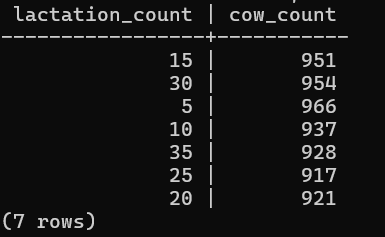
\includegraphics[width=0.5\linewidth]{результаты запросов/5.png}
    \caption{Результат работы запроса 5}
    \label{fig:5}
\end{figure}
\textbf{Время выполнения запроса: }128.990 ms.

На картинке \ref{fig:дер5} представлено графическое представление последовательности выполнения запроса 5.
\begin{figure}[H]
    \centering
    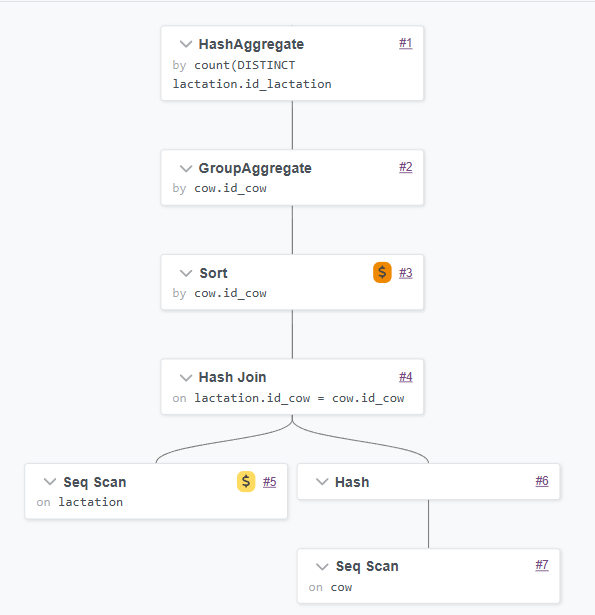
\includegraphics[width=1\linewidth]{деревья/дерево5.png}
    \caption{Графическое представление последовательности выполнения запроса 5}
    \label{fig:дер5}
\end{figure}

\textbf{Текстовое объяснение последовательности выполнения запроса 5.}\\
В данном запросе сначала выполняется вложенный подзапрос, в котором соединяются таблицы \texttt{Cow} и \texttt{Lactation}. Строки группируются по идентификатору коровы (\texttt{GROUP BY Cow.id\_Cow}), а с помощью функции \texttt{COUNT(DISTINCT Lactation.id\_Lactation)} вычисляется количество уникальных лактаций для каждой отдельной коровы. Результат этого подзапроса используется как временная таблица \texttt{cow\_lactations}. Затем во внешнем запросе полученные строки группируются уже по количеству лактаций (\texttt{GROUP BY lactation\_count}), и с помощью функции \texttt{COUNT(id\_Cow)} подсчитывается количество коров, имеющих одинаковое число лактаций.

\textbf{Реляционная формула запроса.}
\[
\mathcal{G}_{\substack{
\text{lactation\_count}, \\
\text{COUNT(cow.id\_Cow)}{\rightarrow}\text{cow\_count}
}} (
\]
\[
\mathcal{G}_{\substack{
\text{cow.id\_Cow}, \\
\text{COUNT(DISTINCT lact.id\_Lactation)}{\rightarrow}\text{lactation\_count}
}} (
\]
\[
\text{Cow} \bowtie_{\text{cow.id\_Cow}=\text{lact.id\_Cow}} \text{Lactation}))
\]


На рисунке \ref{fig:гист5} представлена 2d-гистограмма результатов выполнения запроса 5.
\begin{figure}[H]
    \centering
    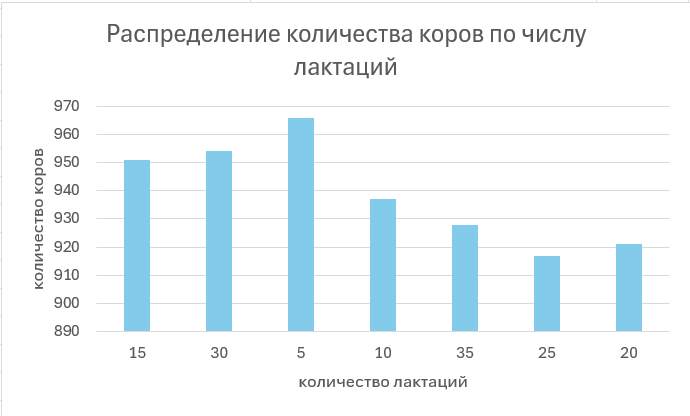
\includegraphics[width=1\linewidth]{гистаграммы/гист5.png}
    \caption{Распределение количества коров по числу лактаций}
    \label{fig:гист5}
\end{figure}

\subsection{Запрос 6}
\textbf{Формулировка запроса на русском языке.}
Найти рационы, по которым питалось больше коров, чем по рациону A.

\listingcaption{Текст запроса 6 на SQL}\label{lst:6}
\begin{Verbatim}[numbers=left, frame=single, breaklines=true, breakanywhere=true]
SELECT Diet.id_Diet, COUNT(DISTINCT Nutrition.id_Cow) AS cow_count
FROM Diet
JOIN Feeding_plan ON Diet.id_Diet = Feeding_plan.id_Diet
JOIN Nutrition ON Feeding_plan.id_Feeding_plan = Nutrition.id_Feeding_plan
GROUP BY Diet.id_Diet 
HAVING COUNT(DISTINCT Nutrition.id_Cow) > (
    SELECT COUNT(DISTINCT Nutrition.id_Cow)
    FROM Diet
    JOIN Feeding_plan ON Diet.id_Diet = Feeding_plan.id_Diet
    JOIN Nutrition ON Feeding_plan.id_Feeding_plan = Nutrition.id_Feeding_plan
    WHERE Diet.id_Diet = 1
);
\end{Verbatim}
На рисунке \ref{fig:6} представлен результат выполнения запроса 6.
\begin{figure}[H]
    \centering
    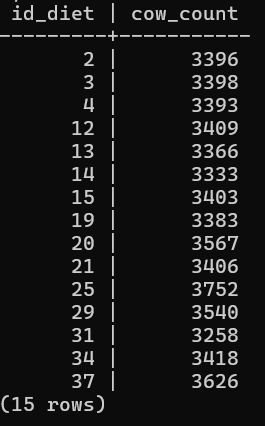
\includegraphics[width=0.5\linewidth]{результаты запросов/6.png}
    \caption{Результат работы запроса 6}
    \label{fig:6}
\end{figure}
\textbf{Время выполнения запроса: }152.362 ms.

На картинке \ref{fig:дер6} представлено графическое представление последовательности выполнения запроса 6.
\begin{figure}[H]
    \centering
    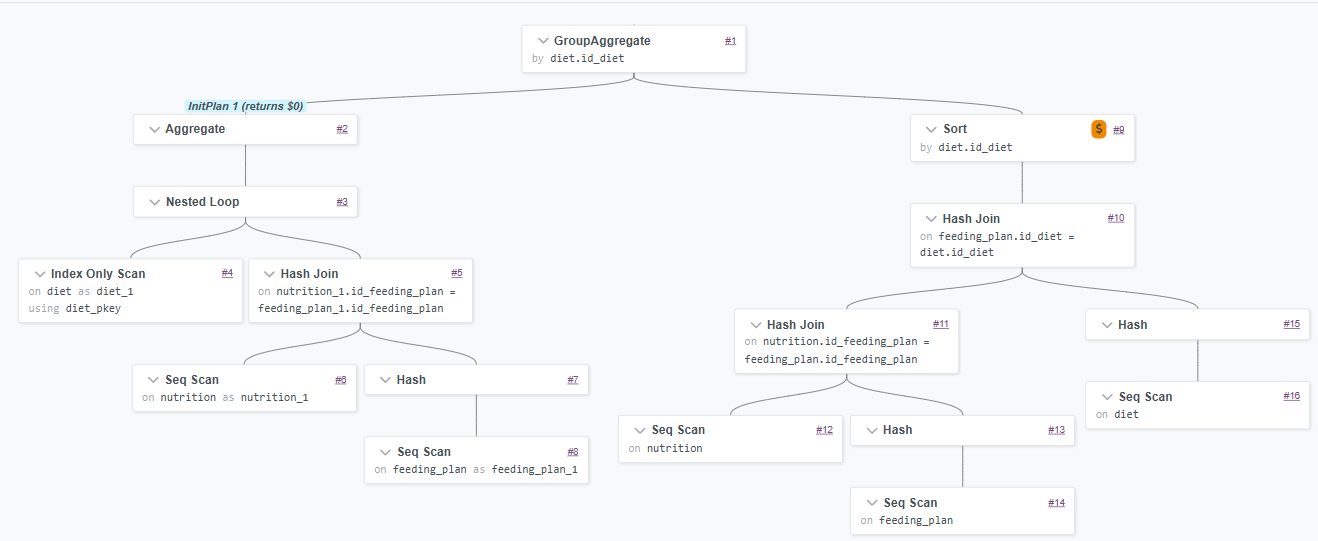
\includegraphics[width=1\linewidth]{деревья/дерево6.png}
    \caption{Графическое представление последовательности выполнения запроса 6}
    \label{fig:дер6}
\end{figure}

\textbf{Текстовое объяснение последовательности выполнения запроса 6.}\\
В запросе последовательно соединяются таблицы \texttt{Diet, Feeding\_plan} и \texttt{Nutrition} с помощью оператора \texttt{JOIN}, после чего строки группируются по идентификатору рациона (\texttt{GROUP BY Diet.id\_Diet}), а функция \texttt{COUNT(DISTINCT Nutrition.id\_Cow)} считает количество уникальных коров для каждого рациона. С помощью условия \texttt{HAVING} выполняется фильтрация сгруппированных данных: количество коров для каждого рациона сравнивается с результатом вложенного подзапроса. Подзапрос вычисляет точное количество уникальных коров, которые питались по рациону с фиксированным идентификатором \texttt{id\_Diet = 1}. В итоговую выборку попадают только те рационы, по которым питалось строго больше коров, чем по первому рациону.

\textbf{Реляционная формула запроса.}
\[
\sigma_{\text{cow\_count} > \text{cow\_count}_{\text{diet.id\_Diet}=1}} (
\]
\[
\mathcal{G}_{\substack{
\text{diet.id\_Diet}, \\
\text{COUNT(DISTINCT n.id\_Cow)}{\rightarrow}\text{cow\_count}
}} (
\]
\[
\text{Diet} \bowtie_{\text{diet.id\_Diet}=\text{fp.id\_Diet}} \text{Feeding\_plan}
\]
\[
\bowtie_{\text{fp.id\_Feeding\_plan}=\text{n.id\_Feeding\_plan}} \text{Nutrition}))
\]


\subsection{Запрос 7}
\textbf{Формулировка запроса на русском языке.}
Найти корма, которые ни разу не попадали в питание коровы A.

\listingcaption{Текст запроса 7 на SQL}\label{lst:7}
\begin{Verbatim}[numbers=left, frame=single, breaklines=true, breakanywhere=true]
SELECT Feeds.id_Feeds, Feeds.Name
FROM Feeds
LEFT JOIN Feeding_plan ON Feeds.id_Feeds = Feeding_plan.id_Feeds
LEFT JOIN Nutrition ON Feeding_plan.id_Feeding_plan = Nutrition.id_Feeding_plan
WHERE Nutrition.id_Cow IS NULL;
\end{Verbatim}

\begin{comment}
На рисунке \ref{fig:7} представлен результат выполнения запроса 7.
\begin{figure}[H]
    \centering
    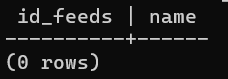
\includegraphics[width=0.5\linewidth]{результаты запросов/7.png}
    \caption{Результат работы запроса 7}
    \label{fig:7}
\end{figure}

\textbf{Время выполнения запроса: }53.750 ms.
\end{comment}

На рисунке \ref{fig:7б} представлен результат выполнения запроса 7.
\begin{figure}
    \centering
    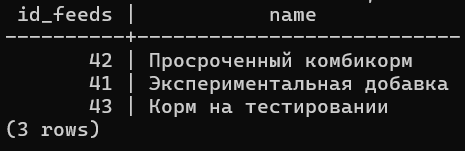
\includegraphics[width=0.5\linewidth]{результаты запросов/7б.png}
    \caption{Результат работы запроса 7}
    \label{fig:7б}
\end{figure}
\textbf{Время выполнения запроса: } 57.780 ms.

На картинке \ref{fig:дер7} представлено графическое представление последовательности выполнения запроса 7.
\begin{figure}[H]
    \centering
    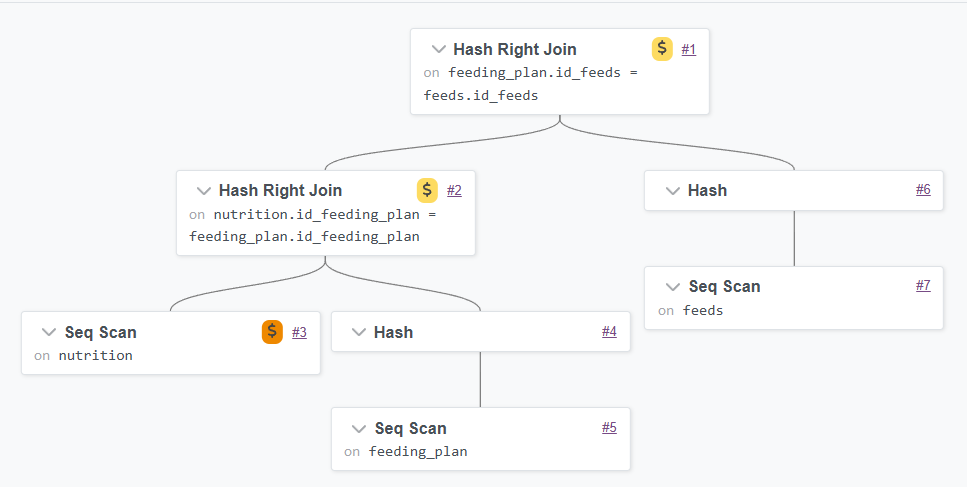
\includegraphics[width=1\linewidth]{деревья/дерево7.png}
    \caption{Графическое представление последовательности выполнения запроса 7}
    \label{fig:дер7}
\end{figure}

\textbf{Текстовое объяснение последовательности выполнения запроса 7.}\\
В запросе к таблице \texttt{Feeds} последовательно присоединяются таблицы \texttt{Feeding\_plan} и \texttt{Nutrition} с помощью оператора внешнего левого соединения \texttt{LEFT JOIN}. Это позволяет сохранить в промежуточной таблице абсолютно все зарегистрированные корма, независимо от того, использовались ли они в планах питания. Затем с помощью условия \texttt{WHERE Nutrition.id\_Cow IS NULL} фильтруются строки и выбираются только те корма, для которых в итоговой таблице отсутствует связь с конкретной коровой. В результате выводятся идентификаторы и названия кормов, которые ни разу не попадали в фактическое питание животных.

\textbf{Реляционная формула запроса.}
\[
\pi_{\text{f.id\_Feeds},\, \text{f.Name}} (
\sigma_{\text{n.id\_Cow IS NULL}} (
\]
\[
\text{Feeds} \underset{\text{f.id\_Feeds}=\text{fp.id\_Feeds}}{\overset{\text{LEFT}}{\bowtie}} \text{Feeding\_plan}
\underset{\text{fp.id\_Feeding\_plan}=\text{n.id\_Feeding\_plan}}{\overset{\text{LEFT}}{\bowtie}} \text{Nutrition}))
\]

 
\subsection{Запрос 8}
\textbf{Формулировка запроса на русском языке.}
Для каждой фазы лактации и породы посчитать число коров.
В результате выполнения запроса получилось 50 записей.

\listingcaption{Текст запроса 8 на SQL}\label{lst:8}
\begin{Verbatim}[numbers=left, frame=single, breaklines=true, breakanywhere=true]
SELECT Lactation_Phase.Name AS Lactation_Phase_Name, Breed.Name AS Breed_Name,
    COUNT(DISTINCT Cow.id_Cow) AS cow_count
FROM Lactation_Phase CROSS JOIN Breed 
LEFT JOIN Cow ON Breed.id_Breed = Cow.id_Breed
LEFT JOIN Lactation ON Cow.id_Cow = Lactation.id_Cow 
    AND Lactation_Phase.id_Lactation_phase = Lactation.id_Lactation_phase
GROUP BY Lactation_Phase.id_Lactation_phase, Lactation_Phase.Name,
         Breed.id_Breed, Breed.Name;
\end{Verbatim}
На рисунке \ref{fig:8} представлен результат выполнения запроса 8.
\begin{figure}[H]
    \centering
    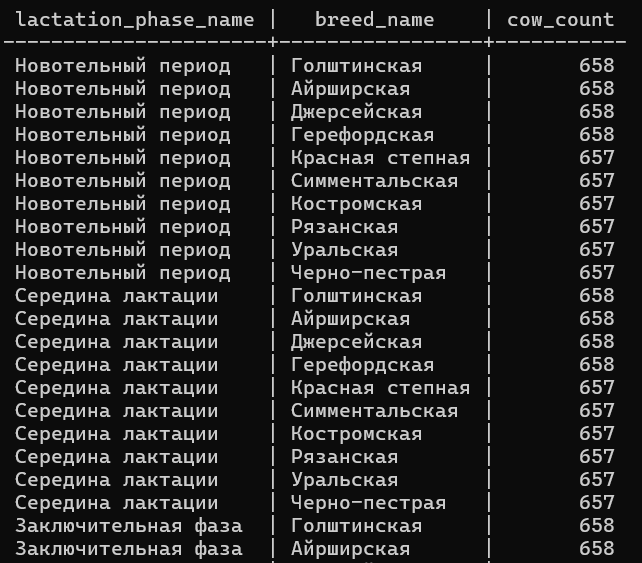
\includegraphics[width=1\linewidth]{результаты запросов/8.png}
    \caption{Результат работы запроса 8}
    \label{fig:8}
\end{figure}
\newpage
\textbf{Время выполнения запроса: }1503.443 ms (00:01.503).

На картинке \ref{fig:дер8} представлено графическое представление последовательности выполнения запроса 8.
\begin{figure}[H]
    \centering
    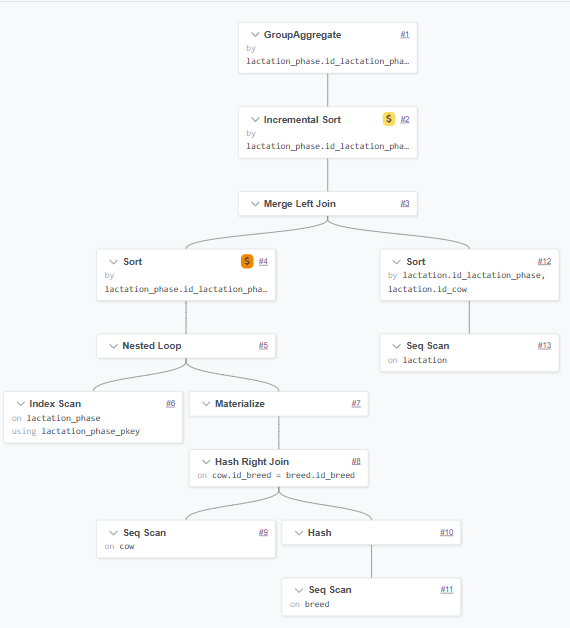
\includegraphics[width=1\linewidth]{деревья/дерево8.png}
    \caption{Графическое представление последовательности выполнения запроса 8}
    \label{fig:дер8}
\end{figure}

\textbf{Текстовое объяснение последовательности выполнения запроса 8.}\\
В данном запросе сначала выполняется перекрестное соединение таблиц \texttt{Lactation\_Phase} и \texttt{Breed} с помощью оператора \texttt{CROSS JOIN}, что позволяет получить декартово произведение, содержащее все возможные комбинации фаз лактации и пород коров. Затем к полученному результату с помощью оператора \texttt{LEFT JOIN} последовательно присоединяются таблицы \texttt{Cow} (по совпадению идентификатора породы) и \texttt{Lactation} (одновременно по идентификаторам коровы и фазы лактации). После этого строки группируются по идентификаторам и названиям фаз и пород. Наконец, с помощью агрегатной функции \texttt{COUNT(DISTINCT Cow.id\_Cow)} вычисляется количество уникальных коров для каждой существующей пары фазы лактации и породы.

\textbf{Реляционная формула запроса.}

\[
\mathcal{G}_{\substack{
\text{lp.id\_Lactation\_phase},\, \text{lp.Name},\, \text{breed.id\_Breed},\, \text{breed.Name}, \\
\text{COUNT(DISTINCT cow.id\_Cow)}{\rightarrow}\text{cow\_count}
}} (
\]
\[
\text{Lactation\_Phase} \times \text{Breed}
\]
\[
\underset{\text{breed.id\_Breed}=\text{cow.id\_Breed}}{\overset{\text{LEFT}}{\bowtie}} \text{Cow}
\]
\[
\underset{\text{cow.id\_Cow}=\text{lact.id\_Cow} \;\wedge\; \text{lp.id\_Lactation\_phase}=\text{lact.id\_Lactation\_phase}}{\overset{\text{LEFT}}{\bowtie}} \text{Lactation})
\]


На рисунке \ref{fig:гист8} приведена 3d-гистограмма результатов выполнения запроса 8.
\begin{figure}[H]
    \centering
    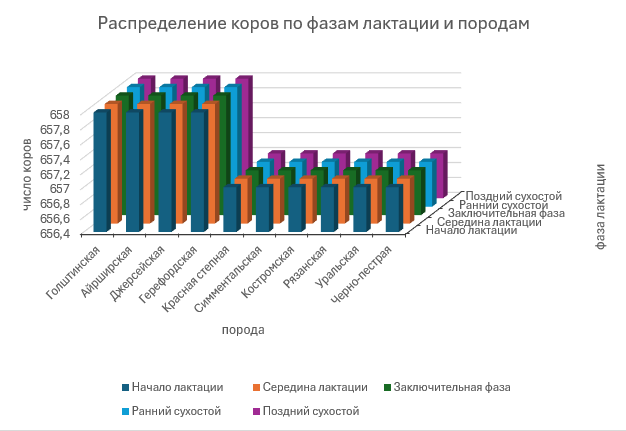
\includegraphics[width=1\linewidth]{гистаграммы/гист8.png}
    \caption{Распределение коров по фазам лактации и породам}
    \label{fig:гист8}
\end{figure}
 
\subsection{Запрос 9}
\textbf{Формулировка запроса на русском языке.}
Во всех рационах заменить зоотехника A на зоотехника B.

\listingcaption{Текст запроса 9 на SQL}\label{lst:9}
\begin{Verbatim}[numbers=left, frame=single, breaklines=true, breakanywhere=true]
UPDATE Diet 
SET id_Livestock_specialist = 1 
WHERE id_Livestock_specialist = 2; 
\end{Verbatim}
На рисунке \ref{fig:9} представлен результат выполнения запроса 9.
\begin{figure}[H]
    \centering
    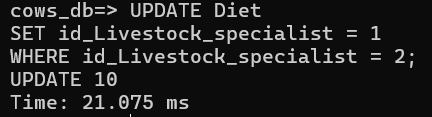
\includegraphics[width=0.5\linewidth]{результаты запросов/9.png}
    \caption{Результат работы запроса 9}
    \label{fig:9}
\end{figure}
\textbf{Время выполнения запроса: }21.075 ms.

На картинке \ref{fig:дер9} представлено графическое представление последовательности выполнения запроса 9.
\begin{figure}[H]
    \centering
    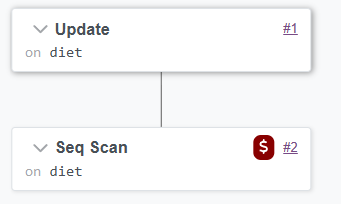
\includegraphics[width=0.5\linewidth]{деревья/дерево9.png}
    \caption{Графическое представление последовательности выполнения запроса 9}
    \label{fig:дер9}
\end{figure}

\textbf{Текстовое объяснение последовательности выполнения запроса 9.}\\
Запрос представляет собой операцию обновления данных с помощью инструкции \texttt{UPDATE}. В таблице \texttt{Diet} для столбца \texttt{id\_Livestock\_specialist} устанавливается новое значение «1» (идентификатор зоотехника Ивана Петрова). При этом с помощью условия \texttt{WHERE} модификация ограничивается только теми строками, где текущий идентификатор зоотехника равен «2» (идентификатор Алексея Иванова). В результате выполнения запроса во всех рационах происходит автоматическая замена ответственного специалиста.

\textbf{Реляционная формула запроса.}
\[
\text{Diet} \leftarrow \pi_{\substack{
\text{diet.id\_Diet},\, \text{diet.id\_Season},\, \text{diet.id\_Lactation\_phase}, \\
\text{1}{\rightarrow}\text{id\_Livestock\_specialist}
}} (
\]
\[
\sigma_{\text{diet.id\_Livestock\_specialist} = 2} (\text{Diet}))
\]
\[
\cup \; \sigma_{\text{diet.id\_Livestock\_specialist} \neq 2} (\text{Diet})
\]